\documentclass[11pt]{article}


\usepackage{mystyle}
\usepackage{emoji}
\setmonofont{SF Mono}
\graphicspath{{src/}}
\usepackage{emoji}
\pagestyle{fancy}
\newcommand{\quotes}[1]{``#1''}
\fancyhf{}
\rhead{HFCS}
\lhead{Lab Manual 3 - Exploring GNU Radio}
\rfoot{\thepage}
\begin{document}

This lab session aims to explore the functionalities of the tool, \mdinlinecode{GNU Radio} which was introduced in Lab 2. \mdinlinecode{GNU Radio} is an open-source toolkit, through which various signal processing blocks of a communication system can be configured and developed in software. These blocks are typically constructed using hardware devices. In \mdinlinecode{GNU Radio}, a system can be made as a flowgraph containing blocks, each of which performs a specific task. Custom blocks can also be programmed using the \mdinlinecode{Python} programming language. \textcolor{red}{It is assumed that all the necessary drivers such as \mdinlinecode{lib-iio}, and \mdinlinecode{gr-iio} etc. have been preinstalled following the steps in Lab manual 2.}

\section{Constructing a simple FSK radio system}

Frequency-shift keying (FSK) is a type of frequency modulation technique in which the digital information is transmitted through a set of discrete frequencies around the centre frequency of the carrier wave. The simplest manifestation of FSK is the binary FSK (BFSK) where two frequencies are used to transmit the bits \mdinlinecode{0} (space frequency) and  \mdinlinecode{1} (mark frequency).

In this section, we will simulate an FSK radio transmitter and receiver by following the steps originally laid out \href{https://wiki.gnuradio.org/index.php/Simulation_example:_FSK}{here}. This will help in familiarising the user interface of the development tool. The end result should appear something like what is shown in Fig. \ref{fig:image2}.


\begin{figure}[!htb]
  \centering
  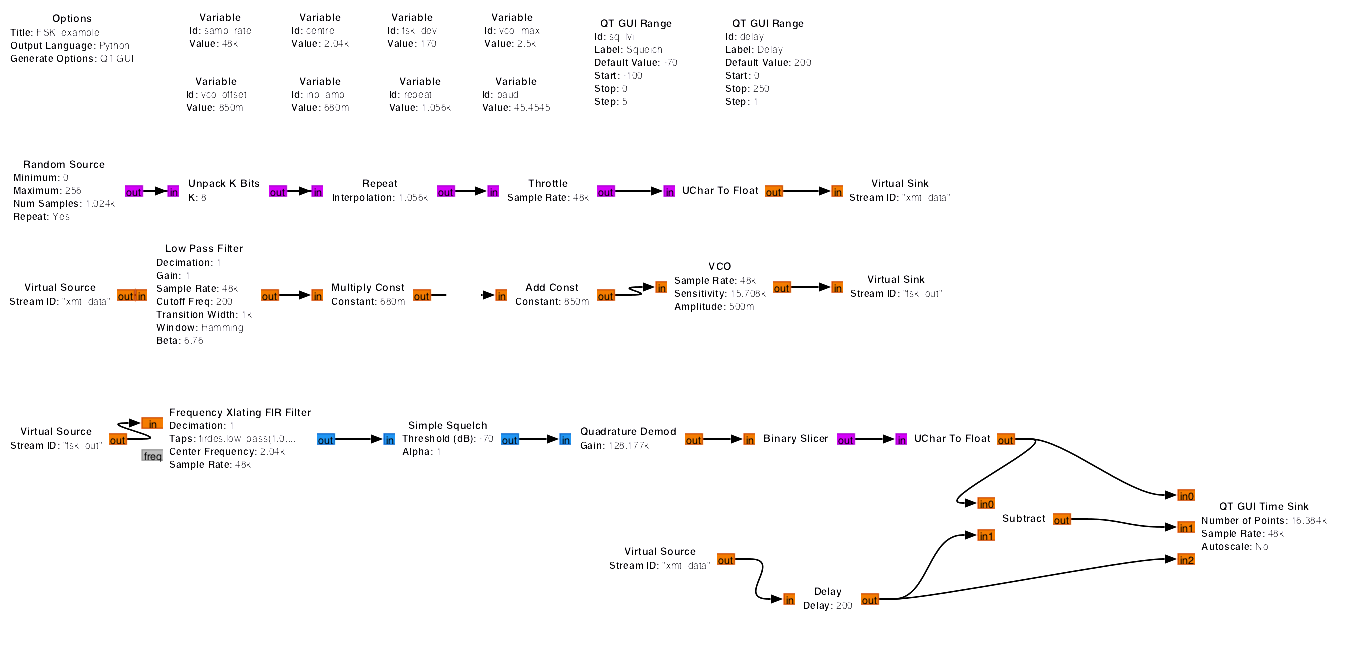
\includegraphics[width=.95\textwidth]{image4.png}
  \caption{FSK Flowgraph in GNU Radio v3.8.}
  \label{fig:image2}
\end{figure}


\subsection{Creating Variables}

Like in any development, the use of variables makes our job easy as the values can be easily reused any number of times. Moreover, if we want to simulate the system in different scenarios, we can easily do so when the variables are present.

Before we begin, it is important to know that there are different types of graphical user interfaces (GUIs) that exist in \mdinlinecode{GNU Radio}. We will use the \mdinlinecode{QT GUI} here. To do so, create a new file by going to \newline \mdinlinecode{File -> New -> QT GUI}. Once you obtain a new blank screen, look for the search icon  (\emoji{mag}) and click it. This will open up a search where different blocks can be quickly inserted.

First, we will insert the \mdinlinecode{Variable} block by dragging and dropping it from the list to the blank space. After double-clicking the variable block, we can configure the \mdinlinecode{id} and \mdinlinecode{value} of each variable.


\begin{tcolorbox}[colback=blue!5]
  \begin{outline}
    \1 Create 8 new variables, the details of each are:
  \end{outline}
  \centering
  \begin{tabular}{|c|c|}
    \hline
    \texttt{samp\_rate}  & 48000   \\
    \texttt{centre}      & 2210    \\
    \texttt{fsk\_dev}    & 170     \\
    \texttt{vco\_max}    & 2500    \\
    \texttt{vco\_offset} & 0.850   \\
    \texttt{inp\_amp}    & 0.680   \\
    \texttt{repeat}      & 1056    \\
    \texttt{baud}        & 45.4545 \\
    \hline
  \end{tabular}
\end{tcolorbox}

The values above suggest a sampling frequency of \SI{48}{\kHz}, the central frequency of the carrier signal \SI{2.21}{\kHz}. The deviation around the chosen central frequency is \SI{170}{\Hz} which determines the frequencies of the mark and space components. These parameters are used in the US version of the Baudot Radioteletype (RTTY). RTTY is a telecommunication system that initially emerged in the late 1800s. Personal computers today are the contemporary manifestation of the RTTYs. The system works on a binary logic (mark and space) and on the transmitter side, FSK is used for modulating the audio tones. In the original (\textit{Baudot}) version of RTTY, 8 bits are used out of which 5 are for data, 1 is for start and 2 are stop bits. The character size is enough to transmit alphabetical letters \mdinlinecode{A-Z} and digits \mdinlinecode{0-9}. A typical RTTY signal is shown in Fig. \ref{fig:image3}. A bit time of \SI{22}{\ms} is used for amateur radio transmissions, which leads to a baud rate:

\begin{align*}
  \text{baud} {}= & \frac{1}{\text{bit \, time}} = \frac{1}{0.022} = \SI{45.4545}{\Hz}
\end{align*}


\begin{figure}[!htb]
  \centering
  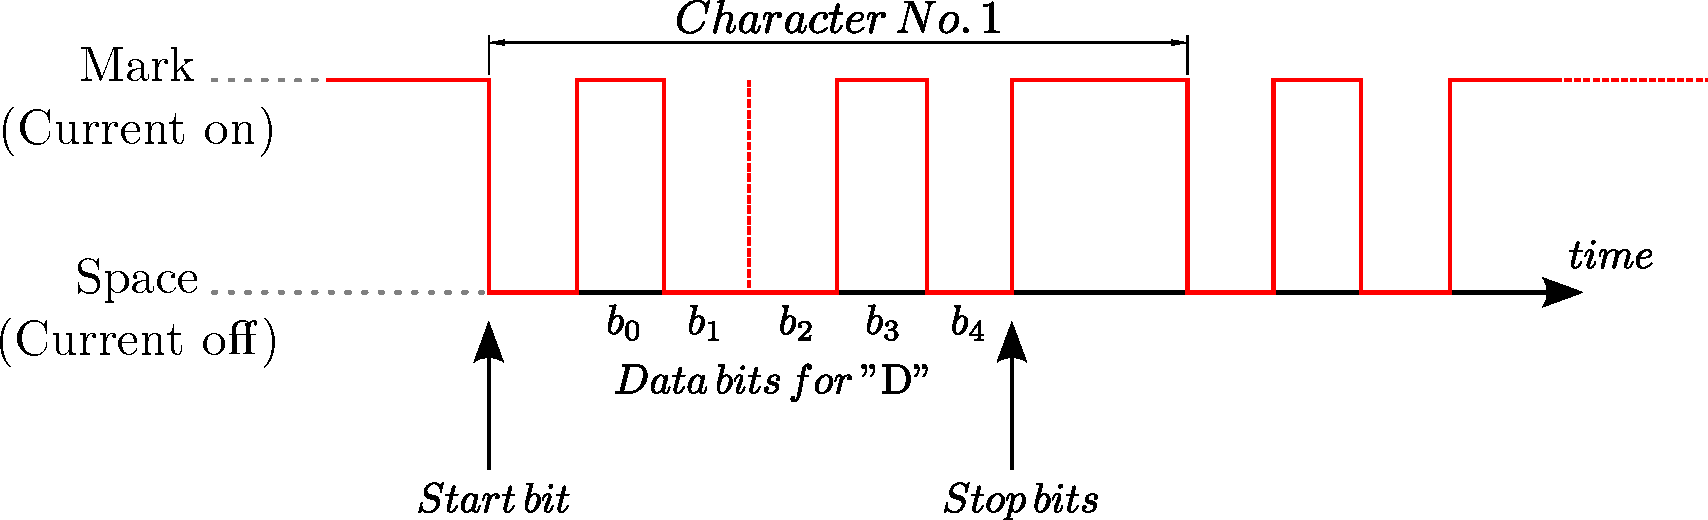
\includegraphics[width=.95\textwidth]{bit stream.pdf}
  \caption{An RTTY data stream for the alphabet D.}
  \label{fig:image3}
\end{figure}

The variable, \mdinlinecode{repeat} refers to the repeat factor which determines the total time of the data frame. In this example, we set it as an integer value:

\begin{align*}
  \text{repeat\, factor} {}= & (\text{int}) \, \mathrm{samp\_rate} \times \mathrm{bit\, time} = 48,000 \times 0.022 = 1056
\end{align*}

In order to select the VCO parameters, we choose a full-scale frequency of \SI{2.50}{\kHz}. Although any value greater than the Mark frequency (in this case, \SI{2.295}{\kHz}) can be chosen, \SI{2.50}{\kHz} is a rounded number.
The delta, $\Delta$ for the VCO is calculated as:
\begin{align*}
  \Delta {}= & \frac{\text{fsk\_dev}}{f_{\mathrm{full-scale}}} = \frac{170}{2500} = \num{0.068}
\end{align*}

The space frequency is created by the:
\begin{align*}
  \text{vco\_offset} {}= & \frac{f_{\mathrm{Mark}}}{f_{\mathrm{full-scale}}} + 0 \times \Delta = \num{0.850}
\end{align*}

Similarly, the Space frequency is created by,
The space frequency is created by the:
\begin{align*}
  \text{inp\_amp} {}= & \frac{f_{\mathrm{Mark}}}{f_{\mathrm{full-scale}}} + 1 \times \Delta = \num{0.918}
\end{align*}

\subsection{Simulating the Transmitter}

The transmitter can be implemented by the following steps:

\begin{outline}[enumerate]
  \1 Create a \mdinlinecode{Random Source} that generates a byte with values ranging from \mdinlinecode{0 - 255}. Ensure that the output type is set to \mdinlinecode{byte}.
  \1 Create a \mdinlinecode{Unpack K bits} block that separates each bit of the input byte and creates a distinct byte out of it. Set the \mdinlinecode{K} value to \mdinlinecode{8}.
  \1 Since we are simulating a virtual source, we would like to limit the data flow. For this, the \mdinlinecode{Throttle} block is created.
  \1 Before we perform any mathematical operations such as filtering, we need to convert the data type of the input stream. We use a \newline \mdinlinecode{UChar to Float} block.
  \1 In order to keep the flowgraph nice, easy to comprehend, we can create a component in multiple lines. We can do this by using the \mdinlinecode{Virtual Sink} and \mdinlinecode{Virtual Source} blocks. These blocks serve as connectors. We need to make sure the \mdinlinecode{Stream ID} matches for a given pair
  \1 For the virtual connectors created above, set the \mdinlinecode{Stream ID} to \newline \mdinlinecode{''xmt\_data''}.
  \1 Next, create a \mdinlinecode{Low Pass Filter} block which reduces the bandwidth the generated signal. The parameters to be entered are, \newline \mdinlinecode{FIR Type - Float - Float (Decimating)}, \mdinlinecode{Decimation = 1}, \newline \mdinlinecode{Gain = 1},  \mdinlinecode{Sample Rate = samp\_rate}, \mdinlinecode{Cutoff Freq = 200}, \newline \mdinlinecode{Transition Width = 1000}, \mdinlinecode{Window = Hamming} and \mdinlinecode{Beta = 6.76}.
  \1 The next involves calibrating the signal to the values so that amplitude is either at the \mdinlinecode{Mark} or \mdinlinecode{Space} frequency voltage levels. For this we use the \mdinlinecode{Const Multiply} and \mdinlinecode{Const Add} blocks for which the Const values are \mdinlinecode{inp\_amp} and \mdinlinecode{vco\_offset} respectively.
  \1 The last step is the most important in which the processed signal is passed to a \mdinlinecode{VCO} block. Here the two voltage levels are converted to the \mdinlinecode{Mark} and \mdinlinecode{Space} frequencies around the centre frequency. The parameters to be inserted are, \mdinlinecode{Sampling Rate = samp\_rate}, \mdinlinecode{Sensitivity = 15708}, and \mdinlinecode{Amplitude = 0.5}.
  \1 Create a \mdinlinecode{Virtual Sink} that is akin to labelling the transmitted signal. We will use it in the receiver module. Use the \newline \mdinlinecode{Stream ID = ''fsk\_out''}.
\end{outline}

The transmitter module should resemble the second and third rows of the flowgraph shown in Fig. \ref{fig:image2}. Note that each block needs to be connected with the adjacent ones. In case there is an error, the arrow becomes \textcolor{red}{red}. Make sure that the data types of each block are the same. Also, note how we have implemented the FSK modulation through the calibration of the VCO.


\subsection{Simulating the Receiver Module}

A typical receiver module in a communication system consists of a filter, demodulation, and conversion components. Let's implement these step by step.

\begin{outline}[enumerate]
  \1 Create a \mdinlinecode{Virtual Source} with to capture the transmitted signal. Make sure to use the same \mdinlinecode{Stream ID} as defined in the transmitter side.
  \1 We now use a \mdinlinecode{Frequency Xlating FIR Filter} block that performs a frequency translation on the received signal. Through this, we can pick up a selected frequency band, translate it to the origin (in this case centre it along the centre frequency), and then remove the remaining frequency components. The parameter values used are, \mdinlinecode{Type = Float - Complex (Complex Taps)}, \mdinlinecode{Decimation = 1}, \newline \mdinlinecode{Taps = firdes.low\_pass(1.0,samp\_rate,1000,400)}, \newline \mdinlinecode{Center Freq = centre}, \mdinlinecode{Sample Rate = samp\_rate}. Here we have utilised the feature to program a block using \mdinlinecode{Python} code.
  \1 Next, create a noise removal \mdinlinecode{Simple Squelch} block that sets a threshold level below which all the signal is removed. Set the \newline \mdinlinecode{Threshold (dB) = 70}, and keep \mdinlinecode{Alpha = 1}.
  \1 The \mdinlinecode{Quadrature Demod} block is used to \textit{demodulate} the received signal. It accepts a complex baseband signal which is then converted into an output, that is the signal frequency in relation to the sample rate, multiplied with the gain. We obtain a signal which is positive for the input frequencies above zero and vice versa. Set the \mdinlinecode{Gain = 128177}.
  \1 The \mdinlinecode{Binary Slicer} module binarises the signal into a byte of \mdinlinecode{1} and \mdinlinecode{0}.
  \1 Create a \mdinlinecode{UChar to Float} module to convert the byte into a numerical value for further processing.
  \1 Create a \mdinlinecode{Virtual Source} with the \mdinlinecode{Stream ID = ''xmt\_data''}, which is followed by a \mdinlinecode{Delay} block having value \mdinlinecode{200}.
  \1 For the purpose of comparison, create a \mdinlinecode{Subtract} block with the inputs coming from the previous two steps.
  \1 To visualise the results, create a \mdinlinecode{QT GUI Time Sink} with three inputs, that come from the last three steps.
\end{outline}

\subsection{Results}

In this section, we require you to paste the results of the simulation created in the sections above.


\begin{tcolorbox}[colback=blue!5]
  Paste the waveform of the transmit and received signals:
  \begin{mdframed}
    \begin{minted}{matlab}
.
.    
.
.
.
.
.
.
.
.
.
.
.
.
  \end{minted}
  \end{mdframed}
\end{tcolorbox}

\section{Exercise}

\begin{outline}[enumerate]
  \1 Plot the frequency spectrum of:
  \2 VCO output
  \2 Xlating FIR Filter
  \2 Digital received signal
  \1 What happens if you change the \mdinlinecode{Centre Frequency} parameter of the \mdinlinecode{Xlating FIR Filter} block to \mdinlinecode{0}?
  \2 Plot the frequency spectrum in this case. Also briefly explain what happens.
  \2 Can you explain WHY do we need to keep the \newline \mdinlinecode{Center Frequency = 2.21 kHz}?
\end{outline}

\end{document}
